\PassOptionsToPackage{xetex}{xcolor}
\PassOptionsToPackage{xetex}{graphicx}
\documentclass[a4paper,landscape,headrule,footrule,xetex]{foils}

%%
%%%  Macros
%%%
\newcommand{\logo}{~}
\MyLogo{HG8011 (2019)}
\newcommand{\Story}{\SHA{HOUN}{The Hound of the Baskervilles}}

\newcommand{\header}[3]{%
\title{\vspace*{-2ex} \large Detecting Meaning with Sherlock Holmes\thanks{Creative Commons Attribution License: you are free to share and adapt as long as you give appropriate credit and add no additional restrictions: 
\protect\url{https://creativecommons.org/licenses/by/4.0/}.}
%\footnotemark
\\[2ex] \Large  \emp{#2} \\ \emp{#3}}
\author{\blu{Francis Bond}   \\ 
\normalsize  \textbf{Division of Linguistics and Multilingual Studies}\\
\normalsize  \url{http://www3.ntu.edu.sg/home/fcbond/}\\
\normalsize  \texttt{bond@ieee.org}}
 \date{Location: LT25}
 \renewcommand{\logo}{#2}
 \hypersetup{
   pdfinfo={
     Author={Francis Bond},
     Title={#2},
     Subject={HG8011: Detecting Meaning with Sherlock Holmes},
     Keywords={Semantics, Pragmatics, Meaning},
     License={CC BY 4.0}
   }
 %  pdfcopyright={Copyright © Francis Bond. Creative Commons 4.0 Attribution License.}
 %  pdflicenseurl={http://creativecommons.org/licenses/by/4.0/}
 }
}
%%
%% Multilingual Stuff
%%
\usepackage[a4paper,landscape,margin=25mm]{geometry}

\usepackage{fontenc}
\usepackage{polyglossia}
\setmainlanguage{english}
\setmainfont{TeX Gyre Pagella}
\usepackage{xeCJK}
\setCJKmainfont{Noto Sans CJK SC}
\setCJKsansfont{Noto Sans CJK SC}
\setCJKmonofont{Noto Sans CJK SC}
%\setCJKttfont{Noto Sans CJK SC}
%\setCJKmainfont{WenQuanYi Micro Hei}
%\clearpage
%\setCJKmainfont{AR PL SungtiL GB}

\usepackage[xetex]{xcolor}
\usepackage[xetex]{graphicx}
\newcommand{\blu}[1]{\textcolor{blue}{#1}}
\newcommand{\grn}[1]{\textcolor{green}{#1}}
\newcommand{\hide}[1]{\textcolor{white}{#1}}
\newcommand{\emp}[1]{\textcolor{red}{#1}}
\newcommand{\txx}[1]{\textbf{\textcolor{blue}{#1}}}
\newcommand{\lex}[1]{\textbf{\mtcitestyle{#1}}}

\usepackage{pifont}
\renewcommand{\labelitemi}{\textcolor{violet}{\ding{227}}}
\renewcommand{\labelitemii}{\textcolor{purple}{\ding{226}}}

\newcommand{\subhead}[1]{\noindent\textbf{#1}\\[5mm]}

\newcommand{\Bad}{\emp{\raisebox{0.15ex}{\ensuremath{\mathbf{\otimes}}}}}
\newcommand{\bad}{*}

\newcommand{\com}[1]{\hfill \textnormal{(\emp{#1})}}%
\newcommand{\cxm}[1]{\hfill \textnormal{(\txx{#1})}}%
\newcommand{\cmm}[1]{\hfill \textnormal{(#1)}}%
\usepackage{amssymb}
\usepackage{relsize,xspace}
\newcommand{\into}{\ensuremath{\rightarrow}\xspace}
\newcommand{\ent}{\ensuremath{\Rightarrow}\xspace}
\newcommand{\nent}{\ensuremath{\not\Rightarrow}\xspace}
\newcommand{\tot}{\ensuremath{\leftrightarrow}\xspace}
\usepackage{url}
\usepackage[hidelinks]{hyperref}
\hypersetup{
     colorlinks,
     linkcolor={blue!50!black},
     citecolor={red!50!black},
     urlcolor={blue!80!black}
}
%\usepackage{hyperxmp}
\newcommand{\lurl}[1]{\MyLogo{\url{#1}}}

\usepackage{mygb4e}
\let\eachwordone=\itshape
\newcommand{\lx}[1]{\textbf{\textit{#1}}}
\newcommand{\ix}{\ex\it}

\newcommand{\cen}[2]{\multicolumn{#1}{c}{#2}}
%\usepackage{times}
%\usepackage{nttfoilhead}
\newcommand{\myslide}[1]{%
\foilhead[-25mm]{\raisebox{12mm}[0mm]{\emp{#1}}}%
\leftheader{}%
\MyLogo{\logo}}

\newcommand{\mytask}[1]{%
\foilhead[-25mm]{\raisebox{12mm}[0mm]{\emp{#1}}}
\leftheader{🔍 Hi}%
\MyLogo{\logo}}

\newcommand{\myslider}[1]{\rotatefoilhead[-25mm]{\raisebox{12mm}[0mm]{\emp{#1}}}}
%\newcommand{\myslider}[1]{\rotatefoilhead{\raisebox{-8mm}{\emp{#1}}}}

\newcommand{\section}[1]{\myslide{}{\begin{center}\Huge \emp{#1}\end{center}}}

\usepackage{tcolorbox}
% \newcommand{\task}{\marginpar{\raisebox{-1ex}{\large
%       \tcbox[colframe=red,colback=white,arc=3pt]{\textbf{?}}}}}
% \newcommand{\task}{\marginpar{\raisebox{-1ex}{
%       \hspace{-0.5em}\tcbox[colframe=red,colback=white,arc=3pt]{%
%         
\includegraphics[width=1.5em]{pics/detective}}}}}
\newcommand{\task}{\marginpar{\raisebox{-2ex}{
      \hspace{-0.5em}\reflectbox{
\includegraphics[width=2em]{pics/detective}}}}}

\usepackage[lyons,j,e,k]{mtg2e}
\renewcommand{\mtcitestyle}[1]{\textcolor{teal}{\textsl{#1}}}
%\renewcommand{\mtcitestyle}[1]{\textsl{#1}}
\newcommand{\chn}{\mtciteform}
\newcommand{\cmn}{\mtciteform}
\newcommand{\iz}[1]{\textup{\texttt{\textcolor{blue}{\textbf{#1}}}}}
\newcommand{\con}[1]{\textsc{#1}}
\newcommand{\gm}{\textsc}
\newcommand{\cmp}[1]{{[\textsc{#1}]}}
\newcommand{\sr}[1]{\ensuremath{\langle}#1\ensuremath{\rangle}}
\usepackage[normalem]{ulem}
\newcommand{\ul}{\uline}
\newcommand{\ull}{\uuline}
\newcommand{\wl}{\uwave}
\newcommand{\vs}{\ensuremath{\Leftrightarrow}~}
%%%
%%% Bibliography
%%%
\usepackage{natbib}
%\usepackage{url}
\usepackage{bibentry}


%%% From Tim
\newcommand{\WMngram}[1][]{$n$-gram#1\xspace}
\newcommand{\infers}{$\rightarrow$\xspace}



\usepackage{rtrees,qtree}
\renewcommand{\lf}[1]{\br{#1}{}}
\usepackage{avm}
%\avmoptions{topleft,center}
\newcommand{\ft}[1]{\textsc{#1}}
%\newcommand{\val}[1]{\textit{#1}}
\newcommand{\typ}[1]{\textit{#1}}
\avmfont{\sc}
%\avmvalfont{\sc}
\renewcommand{\avmtreefont}{\sc}
\avmsortfont{\it}


%%% From CSLI book
\newcommand{\mc}{\multicolumn}
\newcommand{\HD}{\textbf{H}\xspace}
\newcommand{\el}{\< \>}
\makeatother
\long\def\smalltree#1{\leavevmode{\def\\{\cr\noalign{\vskip12pt}}%
\def\mc##1##2{\multispan{##1}{\hfil##2\hfil}}%
\tabskip=1em%
\hbox{\vtop{\halign{&\hfil##\hfil\cr
#1\crcr}}}}}
\makeatletter

\newcommand{\sh}[1]{\lowercase{\href{https://fcbond.github.io/sh-canon/#1.html}}{#1}}
\newcommand{\SHA}[2]{\lowercase{\href{https://fcbond.github.io/sh-canon/#1.html}}{\textit{#2}}}

\usepackage{tikz}
\newcommand{\ili}[1]{\href{http://www.globalwordnet.org/ili/#1}{\url{#1}}}
\newcommand{\todo}{\marginpar{ToDo}}

\newcommand{\tra}[1]{\textcolor{olive}{\textsf{#1}}}
\usepackage{multicol}
\usepackage{booktabs,subscript}
\newcommand{\DF}[1]{\parbox{.6\textwidth}{#1}}
\begin{document}
%\makexeCJKinactive
\renewcommand{\avmvalfont}{\it}
\header{~}{The Annotated Holmes}{\normalsize
  How can we read better?}
%Film Studies and Literature
\maketitle


\myslide{Outline}
\begin{itemize}
\item An online edition of the Canon
\item Teaching through Tagging\\
--- Interactive Lexical Semantics
\item Sense Distributions in NTU-MC
\item Word Sense Disambiguation
\item Sentiment
\item Where do we go from here?
\end{itemize}


\section{An online edition of the Canon}


\myslide{The Adventure of the Readable Texts}
\MyLogo{In the 2017 Beaten Annual, work done with Arthur Bond}
For my students (for this class), I wanted texts

\begin{itemize}
\item faithful to the original
\item easy to read on various devices
\item  aesthetically pleasing
\item linked to the rich world of information of the Great 
Game  
\end{itemize}

Sadly, no one site has given us what we want, so like many
before us, we ended up producing our own.  


\myslide{Data! Data! Data!}
\MyLogo{\eng{“Data! data! data!” he cried impatiently. “I can't make bricks
  without clay.”} \SHA{COPP}{The Adventure of the Copper Beeches (ACD 1892)}}
First, I took a look at what was already out there:

\begin{tabular}{lll}
Edition & Name  \\ %& Misc\\
\hline
Gute      & 
\href{https://www.gutenberg.org/files/1661/1661-h/1661-h.htm#8}{The
           Project Gutenberg HTML} \\
ACD     & 
\href{https://www.arthur-conan-doyle.com/index.php?title=SPEC}{Arthur Conan Doyle Encylopedia}\\
BSW      & 
\href{http://bakerstreet.wikia.com/wiki/The_Adventure_of_the_Speckled_Band}{Baker Street Wiki}\\
SS       & \href{http://www.eastoftheweb.com/short-stories/UBooks/AdveSpec.shtml}{Short Stories}\\
SHC      & \href{https://sherlock-holm.es/stories/html/spec.html}{The Complete Sherlock Holmes Canon}\\
Lit2Go   & \href{http://etc.usf.edu/lit2go/32/the-adventures-of-sherlock-holmes/352/adventure-8-the-adventure-of-the-speckled-band/}{Lit2Go}\\
Camden   &
           \href{http://ignisart.com/camdenhouse/canon/index.htm}{Camden House: The Complete Sherlock Holmes} \\
MoonFind & \href{http://mrmoon.com/moonfind/holmes/}{MoonFind: Searching for Sherlock}
\end{tabular}


\myslide{Selection Criteria}
\MyLogo{
  \textit{‘It has long been an axiom of mine that the little things are infinitely the most important.’}
A Case of Identity}

\begin{itemize}
\item Useful Metadata: When and where published, Author, Copyright,
  \ldots
\item Annotation:  links to TV and film
versions, chronologies, definitions of words and Sherlockian
scholarship
\item Spoilers!  Does the annotation reveal the villain?
\item Font: Is it a nice serif font (like in the Strand Magazine)
\item Resizability: can you read it on your phone
\item Pictures: does it have the illustrations nicely embedded?
\item Miscellaneous:  does it have search?

\end{itemize}


\myslide{Results}


\begin{table}
\caption{Rating Online Texts of the Canon}
\bigskip
\label{tab:editions}
\begin{tabular}{lccccccl}
Edition & Meta & Annotation & Spoilers & Font & Resize & Pics & Misc\\
\hline
ACD    & A & A & F & C & F & C & Search\\
Gute   & C & F & - & A & A & F & Book \\
BSW    & A & A & F & B & F & F & Ads \\
SS     & C & F & - & C & A & F & Ads \\
SHC      & C & F & - & A & B & F & ToC \\
Lit2Go   & A & F & - & C & F & F & Audio \\
Camden   & A & F & - & C & F & A & ToC \\
MoonFind & F & F & - & C & F & F & Search 
\end{tabular}
\end{table}

Every site had some good points, but no one is perfect.

\myslide{Our Approach}
\MyLogo{\textit{‘There is nothing new under the sun. It has all been done before.’}
A Study in Scarlet}
\begin{center}
  \url{http://compling.hss.ntu.edu.sg/canon}
\end{center}

\begin{itemize}
\item Resizable, nice font with tufte-css
\item Full table of contents, linked from each story
\item Metadata in the margin: the date and place of publication, story
  number, which collection, \textit{date of action?}
\item Illustrations in the text\todo 
  % \begin{itemize}
  % \item From the Victorian web (more available)
  % \end{itemize}
\item Links to annotation at the end
  \begin{itemize}
  \item Wikipedia
  \item Arthur Conan Doyle Encylopedia
  \item Bill Dolan's Study Guide
  \end{itemize}
\end{itemize}

\myslide{Annotation (new + ToDo)}
\begin{itemize}
\item Locations link to google maps
  \begin{itemize}
  \item What should we do for made-up places?\task
  \item Should link locations to geonames\todo
  \end{itemize}
\item Currency links to amount in today's currency
  \\ done for \sh{SPEC}
\item Person + Organization should link to entry in ACD Encylopedia
\item  Texts are searchable with a site-specific google search
  \\ metadata is hidden from indexing by the \texttt{<!--googleoff: all-->} command.
\end{itemize}


\myslide{Annotation ToDo}

 \begin{itemize}
  \item The sense level annotations of the \textit{NTU Multilingual Corpus}, which links each open class word to its definition in Wordnet%\footnote{{http://compling.hss.ntu.edu.sg/ntumc/cgi-bin/showcorpus.cgi}}
    \begin{itemize}
    \item We can also show translations and/or hypernyms
    \end{itemize}
  \item Content level annotation like the Annotated Sherlock Holmes

  \item We have syntactic annotation (treebanks) for \textit{The Adventure of the Speckled Band} which it would be good to display for those who are interested

  \item More from the \href{http://www.beaconsociety.com/}{Beacon
      Society}'s award winners, including information about word
    meaning, rhetorical devices, \ldots

  \item Links to facsimiles of the original stories

\end{itemize}

\myslide{Translations and Glosses}

\begin{itemize}
\item The Canon has been widely translated: we would like to also
  prepare editions of foreign languages, and consider the issue of
  linking the translations.  E.g.,   \href{https://inlector.wordpress.com/2013/01/15/the-adventures-of-sherlock-holmes/}{\textit{InLéctor}},
  who have produced a nice bilingual English-Spanish edition of
  \textit{The Adventures of Sherlock Holmes}.

\item With the multilingual wordnets, we can present glosses of the
  correct sense, in any of 34 languages (although not all will be
  complete)

\item We can investigate how to choose the words to highlight
  \begin{itemize}
  \item Low frequency (rare) word
  \item Lower frequency sense of a word (uncommon meaning)
  \item No direct translation --- give definition
  \item Word selected by e.g., Bill Dolan, my students, \ldots
  \end{itemize}
 it is quite hard to do this nicely, ... 

\end{itemize}

\myslide{Some Technical Issues}

\begin{itemize}
\item There is a lot of duplication in online resources (and I have
  only made it worse)

\item How can we share information?
  \begin{itemize}
  \item Put the code and meta-data on github
\begin{verbatim}
SPEC	PUBLISHED	The Strand Magazine in February 1892
SPEC	ORDER	10
SPEC	COLLECTION	The Adventures of Sherlock Holmes
SPEC	DORN	http://www.beaconsociety.com/uploads/3/7/3/8/37380505/dorn_spec_study_guide.pdf
SPEC	TITLE	The Adventure of the Speckled Band
SPEC	IMAGE	She lifted her veil	104.jpg
\end{verbatim}
    are there standard ways to refer to lines? 
  \end{itemize}
\item Is everyone happy to share information?
  \begin{itemize}
  \item We have to make sure not to use data without permission
  \end{itemize}
\end{itemize}


% \myslide{Acknowledgements}

% We would like to thank the Sound of the Baskervilles for their
% encouragement and advice; Alexis Barquin of the Arthur Conan Doyle
% Encyclopedia, who kindly allowed us to access his database of texts;
% and the makers of all the many editions we read --- we learned
% something from all of them.


\myslide{Conclusion}

\begin{itemize}
\item We now have some stories with every (open-class) word linked to
  an entry in a dictionary, and its grammatical category \\ What else can
  we do with this?
\item For \sh{SPEC} we also have this in Chinese, Japanese, Indonesian,
  Italian (and are working on Abui, Bulgarian, Dutch, Spanish and
  Polish).  And these are linked to the English
  \\ What we can do with this?
\item If you have any ideas (or want the data, or want to help me make
  more) please let me know.

\end{itemize}



\myslide{The Canon for Learners}

There are some nice versions annotated for non-English speakers.


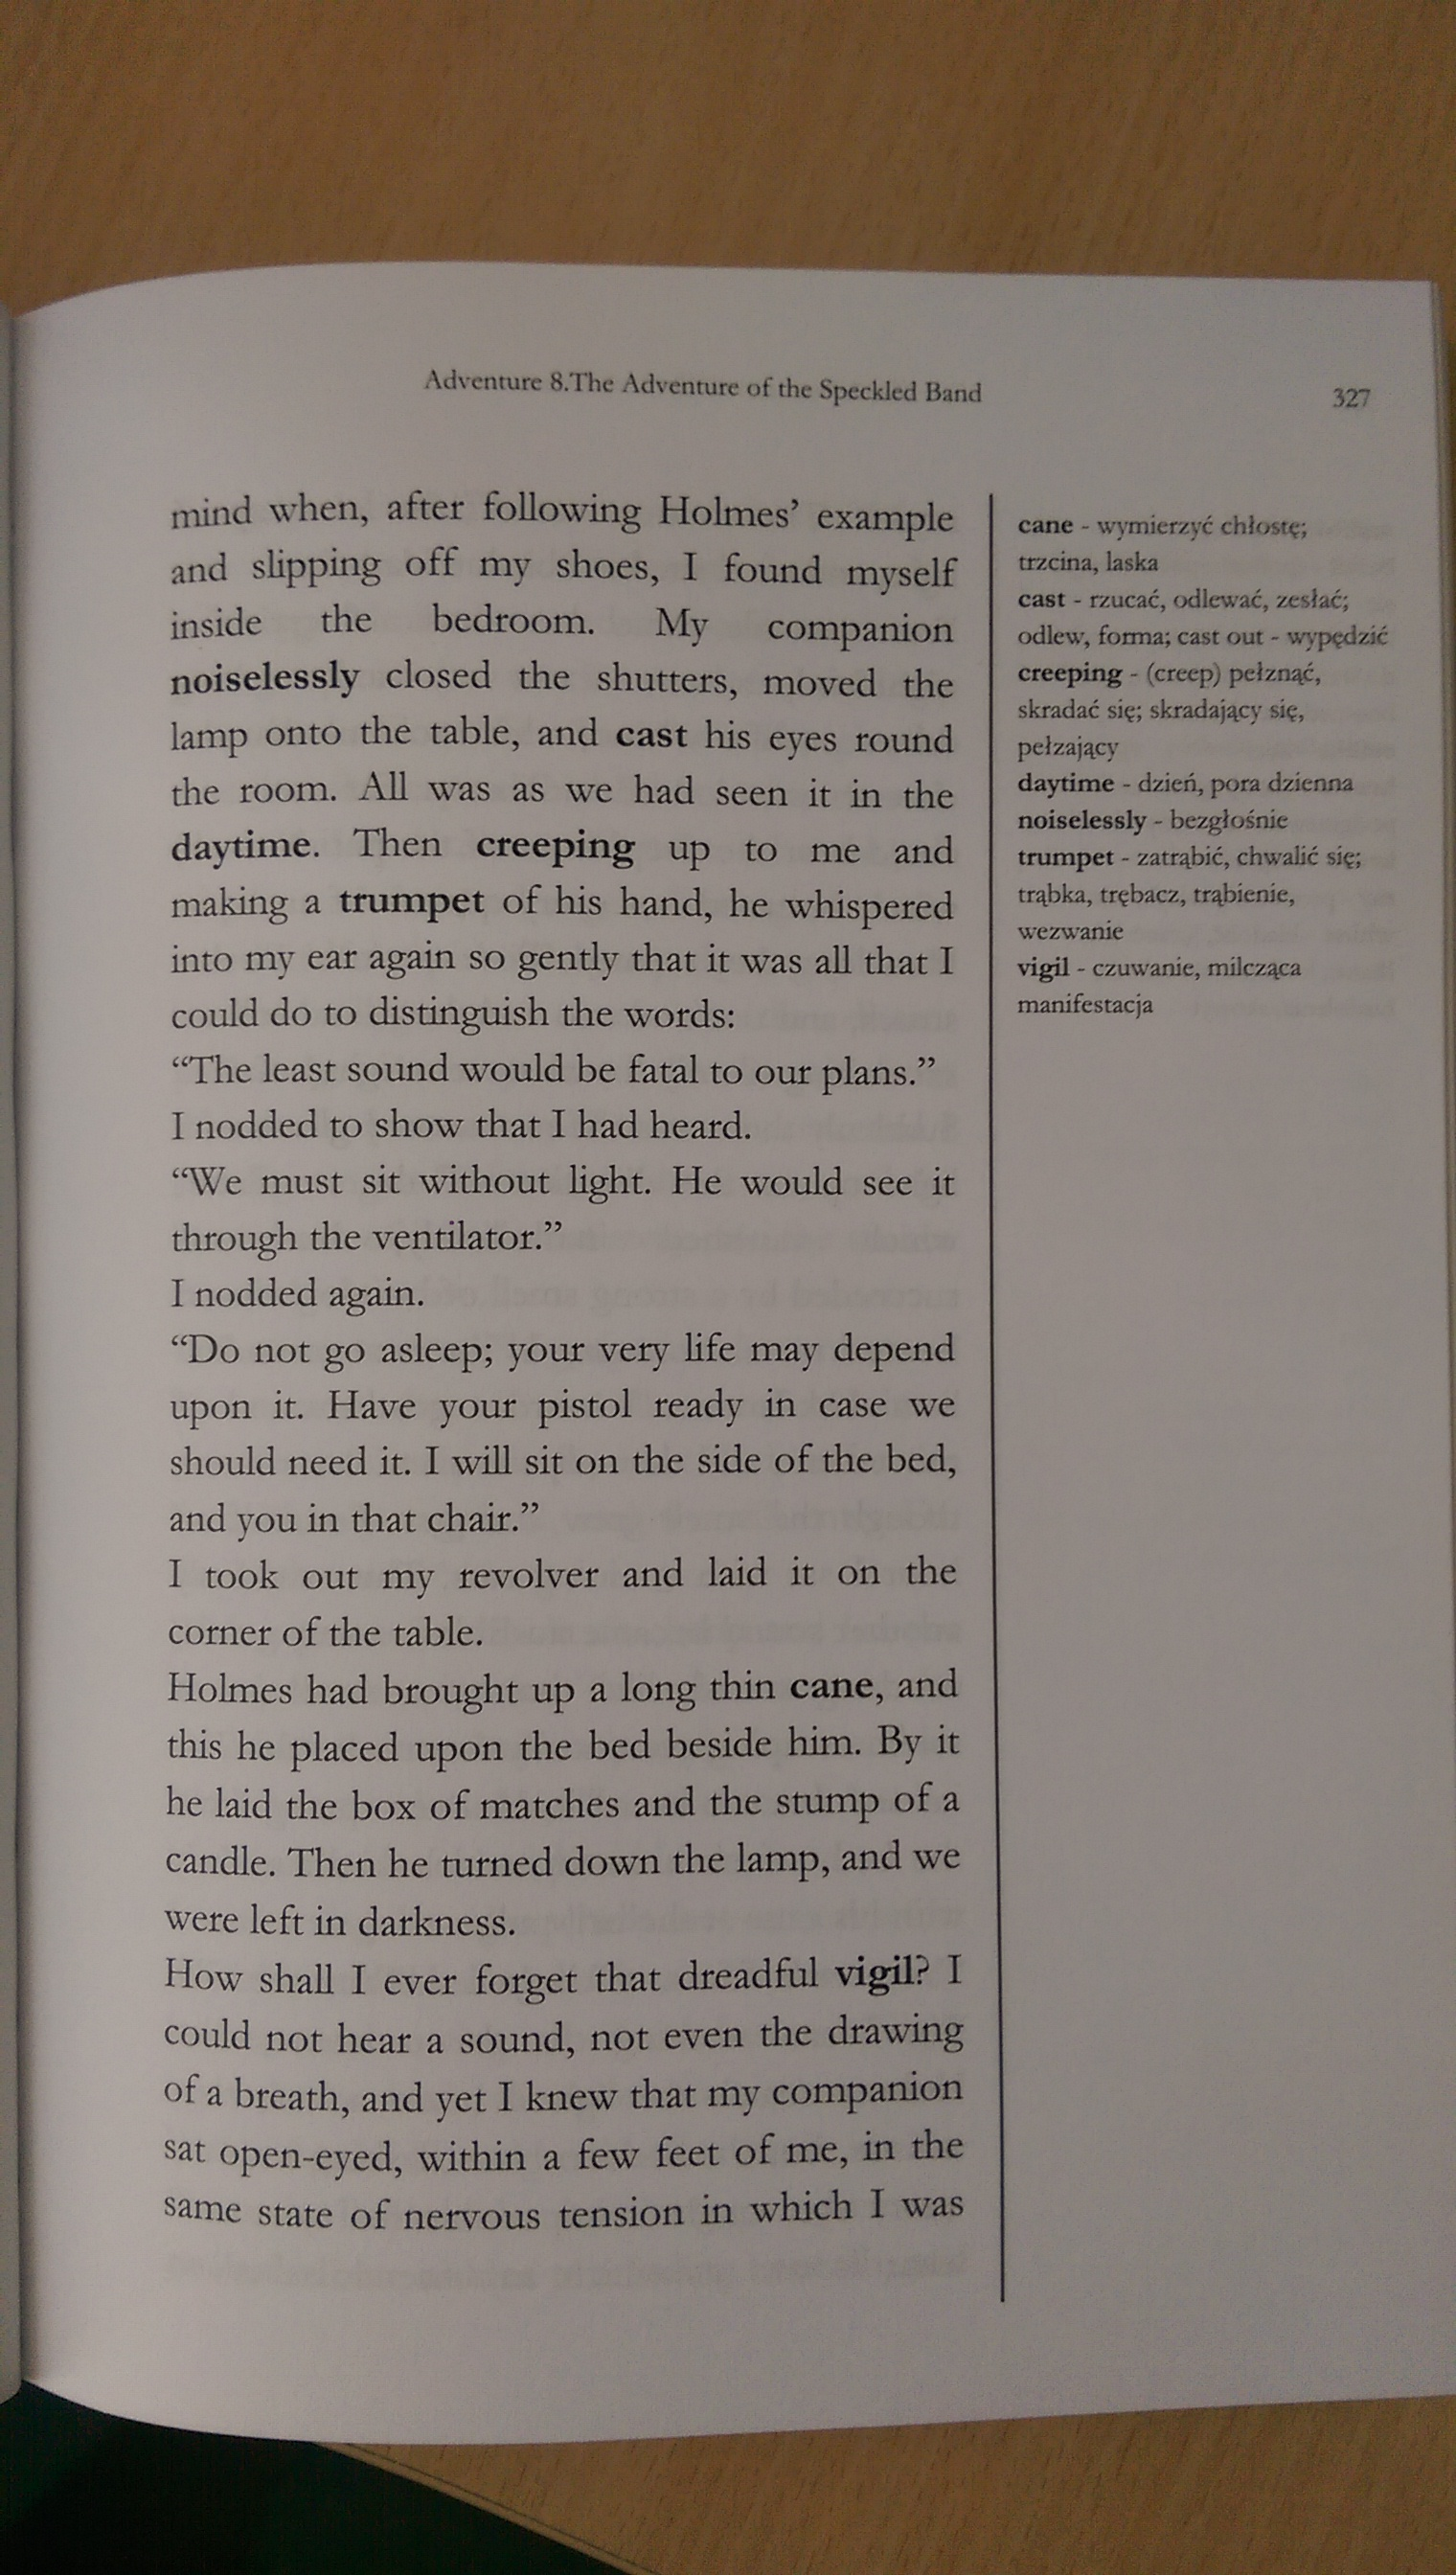
\includegraphics[trim={0 48cm 0 16cm},clip,width=\textwidth]{IMAG0172}



\myslide{The Canon for Learners: problems}

\begin{itemize}
\item \emp{BUT}, the glosses are not very good.  The correct sense is not
  highlighted (or sometimes even listed)
    \begin{itemize}
    \item \textbf{cane} --- whip$_v$; reed$_n$, \ul{cane$_n$}
    \item \textbf{cast} ---  throw$_v$, make forms$_v$, send out$_v$,
      cast ou$_v$t; metal cast$_n$, form$_n$
      \\ should be \eng{cast one's eyes} ``take a quick look''
    \item \textbf{crane} --- mechanical crane
      \\ should be \eng{Crane Water} ``place name''
    \item \textbf{masonry} --- ``The occupation or work of a mason''
      \\ should be \eng{stonework}
  \end{itemize}
\item It is not clear how the words are selected
\\ Why not \textbf{dog-cart, homely, spring up, stump}?
\item With our sense tags we can do better than this!
\end{itemize}



\section{Teaching through Tagging}

\myslide{Teaching Meaning to my Students}
\MyLogo{some of the things I make/let my students do}

\begin{itemize}\addtolength{\itemsep}{-1ex}
\item Read a Sherlock Holmes story
  \begin{itemize}
  \item  So far \sh{SPEC}, \sh{DANC}, \sh{REDH} and \sh{SCAN}
\\ (also news, essays and Japanese short stories)
  \end{itemize}
\item Look at every content word
  \begin{itemize}
  \item Find its meaning in a dictionary (wordnet)
  \item Or write a new definition if needed
  \item Say if it has positive or negative connotation (for some)
  \end{itemize}
  this shows how little you need to know to understand and enjoy
\item Rewrite it using only the most common 1,000 words of English
  \begin{itemize}
  \item Like XKCD's \href{https://xkcd.com/simplewriter/}{Simple Writer}
    (used in \textit{Thing Explainer})
  \item We only did this for \sh{REDH}
  \end{itemize}
  this also shows some interesting misunderstandings
\end{itemize}


%\section{Word Meaning Revisited}

\myslide{Defining Meaning}

\begin{itemize}\addtolength{\itemsep}{-1.5ex}
\item When we use a word, we don't have to know everything about the
  referent
  \begin{itemize}
  \item A \eng{dog-cart} is a kind of \con{cart}
  \item[\ent] you can ride it
  \item[\ent] it has wheels
  \item[\ent] it has something to do with a dog
  \end{itemize}
\item We infer that it has many of the same properties as its
  hypernym, even though this is not always true
 \begin{itemize}
  \item A \eng{hover-car} is a kind of \con{car}
  \item[\ent] you can ride it
  \item[$\not\Rightarrow$] it has wheels
  \end{itemize}
\item Many of the properties may be irrelevant to the story at hand,
  and irrelevant to the syntax of the language
\end{itemize}

\myslide{How do we learn?}
\vspace*{-1ex}
\begin{quote}
  \textit{You shall know a word by the company it keeps} \hfill
\citep[p11]{Firth:1957}
\end{quote}
\vspace*{-1ex}
\begin{itemize}\addtolength{\itemsep}{-2ex}
\item You see a new word \emp{in context}
\\ \eng{buttoning up his \ul{pea-jacket}, }
\begin{itemize}
\item[\ent] it is a kind of jacket \hfill(\eng{green jacket}?)
\item[\ent] with buttons
\item [?] it is thick material (they are going to a stake out)
\item[?] it has something to do with peas \\ not true (from the West
  Frisian word \eng{pijjakker}, in which \eng{pij} referred to the
  type of cloth used, a coarse kind of \ul{twilled} blue cloth)
\end{itemize}
\item And you deduce information from the context
\item We are getting better at doing this with computers
\begin{itemize}
\item but people use more than words: eyes, noses and other senses
\end{itemize}

\end{itemize}

\myslide{How else do we learn?}

\begin{itemize}\addtolength{\itemsep}{-1.5ex}
\item From word internal cues
  \begin{itemize}
  \item \eng[far vision]{Television} 
  \item \eng[internet phone]{iphone} 
    (also individual, instruct, inform, inspire)
  \item 鯖 \jpn[mackerel]{saba} = 魚 fish; 青 blue
  \end{itemize}
\item From the sound
  \begin{itemize}
  \item \eng{bouba/kiki}  $\star$ or $\clubsuit$
  \item \eng{banged, beaten, battered, bruised, blistered, bashed}
  \item mouth shape for \eng{teeny weeny} vs \eng{large}
  \end{itemize}
\item From  images:
  \begin{tabular}[t]{c}

\includegraphics[width=4em]{pics/magnifying-glass} \\    
 \eng{Magnifying Glass} 
  \end{tabular}
\end{itemize}


\myslide{Words are related in many other ways}


\begin{itemize}
\item Domains: \eng{ball, racket, net, love, ace}
\item Origin: \eng{chew, eat, drink} vs \eng{masticate, consume, imbibe}
\item[?] come up with some words with different origins\task 
  \\ English or another language!
\item Dialect: \eng{ripper, bonza, sickie, no worries}
\item Part-of-speech: \eng{die, live} vs \eng{death, life}
\item When you learned them!
\item and many more
\end{itemize}

All of these relations affect how you use and understand language.

\myslide{Idioms}

\begin{itemize}
\item Some expressions clearly involve more than one orthographic word
  \begin{itemize}
  \item compound noun
    \begin{itemize}
    \item \eng{\ul{grass snake}}; \eng{\ul{grass} and \ul{tree} \uuline{snakes}}
    \end{itemize}
  \item verb-particle
    \begin{itemize}
    \item \eng{I \ul{looked} it \ul{up}} vs \eng{I \ul{looked up} the very long word}
    \end{itemize}
  \item  idiom
    \begin{itemize}
    \item \eng{\ul{going great guns}, \ul{give the Devil his due}}
    \item \eng{\ul{jog someone's memory}}
    \item \eng{\ul{blow one's top}}, \eng{\ul{cast one's eyes}}
    \end{itemize}
% \item And more
% \\ \eng{San Francisco, ad hoc, by and large, Where Eagles
% Dare, kick the bucket, part of speech, in step, the
% Oakland Raiders, trip the light fantastic, telephone
% box,  take a walk , do a number on
% (someone), take (unfair) advantage (of), pull strings,
% kindle excitement, fresh air, \ldots}
  \end{itemize}
\item Knowing the individual words is not enough to know the meaning (or usage)
  
\end{itemize}

% \myslide{Multiword Expressions (MWE)}

% There are many different kinds of irregularity.

% \begin{tabular}{lccccc}
%   MWE & \multicolumn{5}{c}{Weirdness} \\
%                   & Lex  & Syn & Sem & Prag & Stat \\
% \hline
% \eng{ad hominem}       &  $+$ & ?   &  ?   &   ?   & $+$ \\
% \eng{at first}          &      & $+$ &     &      & ? \\
% \eng{first aid}         &      &      & $+$   &      & ? \\
% \eng{salt and pepper}   &      &      &      &      & $+$\\
% \eng{good morning}      &      &      &      &  $+$ &$+$ \\
% \eng{cat's cradle}     & $+$  &      &  $+$ &      & ?\\
% \end{tabular}

% \begin{itemize}
% \item Most of the time, we don't even notice
% \item Unless it is your second language
% \item In Project 4 you will try to find examples of interesting
%   multi-word expressions
% \\ from a new story
% \end{itemize}

\myslide{How common are MWEs?}

\begin{itemize}
\item They are very common in the lexicon
  \begin{itemize}
  \item In wordnet,  41\% of the entries are multiword %(mainly compound nouns)
  \end{itemize}
\item But less common in the actual text (\sh{SPEC} 4.5\%: 296/6,641)
\\ 24 are new (not in Wordnet 3.0); 55 are named entities
% sqlite3 /var/www/ntumc/db/eng.db "select substr(tag,1,1), clemma, tag, count(clemma) from concept where sid >=11000 and sid <=11700 and tag != 'x' and clemma glob '* *' group by substr(tag,1,1)"
% -- Loading resources from /home/bond/.sqliterc

% substr(tag,1,1)	clemma	tag	count(clemma)
% 0	and so	00117620-r	206
% 1	good fortune	11463746-n	11

% 7	no one	77000137-n	3
% 8	pull off	80000623-v	16
% 9	last night	90000518-n	5

% d	four o'clock	dat	1
% l	baker street	loc	18
% o	in order	oth	3
% p	Hilton Cubitt	per	32
% w	as well as	w	1

  \begin{itemize}
  \item \eng{take into one's confidence}
  \item \eng{take in}
  \item \eng{Sherlock Holmes}
  \item \eng{practical joke(r)}
  \item \eng{in love}
  \item \eng{get the better of}
  \item \eng{Panama hat}
  \item \eng{as good as one's word} 
  \end{itemize}
%\item It still seems as though we are missing many MWEs
\end{itemize}

\myslide{Why are they important?}

\begin{itemize}
\item If you think you know the individual words, then you might be  confused

\item Which is a problem if you are a translator:
\\ \eng[whoever he met]{whoever crossed his path} \sh{SPEC}
\\ 私道を渡ろうとする人 ''whoever tried to cross his private road''
\item Knowledge of MWEs is one of the things that separates a good speaker from a poor one
\item From a linguist's point of view, they also reveal something about
  how language is organized in our brains
\end{itemize}

% \myslide{Metaphors in Sherlock Holmes}
% \begin{exe}
  
% \ex \eng{"Oh, sir, do you not think that you could help me, too, and  and at least \ul{throw a little light} through \ul{the dense darkness which surrounds me}"}
% %\ex \eng{"You may advise me how to \ul{walk amid the dangers which encompass me.}"}
% \ex \eng{" 'Tell me, Helen,' said she, 'have you ever heard anyone whistle \ul{in the dead of the night}?"}
% \ex \eng{"my sister was quite alone \ul{when she met her end}"}
% \ex \eng{"My companion sat in the front of the trap, his arms folded, his hat pulled down over his eyes, and his chin sunk upon his breast, \ul{buried in the deepest thought}"}
% %\ex \eng{"As we passed out he exchanged a few words with the landlord, explaining that we were going on a late visit to an acquaintance, and that it was possible that \ul{we might spend the night there}."}
% \ex \eng{"The presence of the gypsies, and the use of the word `band', which was used by the poor girl, no doubt to explain the appearance which she had caught a hurried glimpse of by the light of her match, were sufficient to \ul{put me upon an entirely wrong scent}."}
% \end{exe}


\section{Sense Distributions in NTU-MC}

\myslide{Cross-lingual comparison}

We consider a single Sherlock Holmes story \textit{The Adventure of
  the Speckled Band}\citep{Doyle:1892} in the original English and
translations in Mandarin Chinese, Indonesian and Japanese \citep[NTU Multilingual Corpus:][]{Tan:Bond:2012}.  The senses
are tagged with the Princeton Wordnet of English
\citep{_Fellbaum:1998}, the Chinese Open Wordnet
\citep[see][]{Wang:Bond:2013}, the Wordnet Bahasa
\citep{Bond:Lim:Tan:Riza:2014} and the Japanese
wordnet\citep{Isahara:Bond:Uchimoto:Utiyama:Kanzaki:2008} enhanced
with pronouns, exclamatives and classifiers
\citep[COW: ][]{Seah:Bond:2014,daCosta:Bond:2016}.  On the basis of wordnet
alignment within the Open Multilingual WordNet
\citep{Bond:Foster:2013}, we are able to compare the distribution of
senses across languages.   

\begin{table}[tbp]
  \centering
\begin{tabular}{lrrrrr}
\hline
 Language   &   Sentences &   Words &   Concepts &    MWC & SWC   \\
\hline                                                            
 English    &         599 &   11741 &        6425 &   285 & 6140  \\
 Indonesian &         709 &   10345 &        6140 &   279 & 5861  \\
 Japanese   &         702 &   13936 &        4925 &   174 & 4751  \\
 Mandarin   &         619 &   12681 &        8263 &   316 & 7947  \\
\hline
\end{tabular}
 
  \caption{Corpus size per language}
  \label{tab:size}
\end{table}

\newpage

\begin{table}[tbp]
  \centering
\begin{tabular}{lrrrr}
%\hline
            & \multicolumn{3}{c}{Ambiguity} & Variation \\
 Language   &   Lexical & Corpus  &   Maximum & Maximum \\
\hline
 English    & 1.33   &    1.26 &              10 &               4 \\
%(/ 206.941 155.287) 1.332635700348387
 Indonesian & 2.88   &    1.15 &              11 &               7 \\
% (/ 106.688  36.954) 2.88704876332738
 Japanese   & 1.68   &    1.05 &               9 &               7 \\
% (/ 158.058  93.834) 1.684442739305582
 Mandarin   & 1.30   &    1.01 &               9 &              10 \\
% (/  79.809 61.533 ) 1.2970113597581785
%\hline
\end{tabular}
 \caption{Ambiguity per language}
  \label{tab:ambi}
\end{table}
\begin{itemize}
\item Lexical Ambiguity
  \begin{itemize}
  \item Indonesian is high as we record both suffixed and root forms: 
    \lex{igal}, \lex{mengigal} ``dance'' (will treat as variants in OMW
2.0)
\item Japanese is high due to character variation
  and multiple scripts: \\ \jpn{檜, 桧, ひのき, ヒノキ} \jpn[Japanese
  cedar]{hinoki} (variants)
\end{itemize}
\item Corpus ambiguity
  \begin{itemize}
  \item Much closer
  \item Japanese and Chinese less ambiguous
  \item [$\Rightarrow$] ★ due to the Chinese characters ★%(we hypothesize)
  \end{itemize}
\end{itemize}
% \begin{itemize}\addtolength{\itemsep}{-1.5ex}
% \item  The one sense per discourse hypothesis \citep{Gale:1992:OSP:1075527.1075579}
% definitely does not hold 
% \item  The most ambiguous words in
% English are \lex{see}, \lex{so}, and \lex{be}.
% \item Verbs and adverbs are the most polysemous in all languages
% \item Interesting variation is the average
% ambiguity: Chinese and Japanese which are written using Chinese
% characters show far less ambiguity than English and Indonesian:
% \\  The
% more complicated orthography reduces ambiguity. 
% \item  At the peaks: how
% ambiguous is the most ambiguous lemma, and how many ways are there to
% represent the most varied concept (variation), there is less
% difference between languages.
%\end{itemize}

\myslide{One Sense Per Discourse}
 \begin{itemize}
  \item Gale hypothesized that a
    single word would tend to have a single sense within a given
    discourse. 
  \item   This was definitely not the case here, in any language.
  \item We get from 9--11 different meanings, with (light) verbs and adverbs
    being most ambiguous --- more true for nouns
    \begin{itemize}
    \item en: \lex{see, be, so, make, have}
    \item ja: \lex{ある, 分かる, 持つ, 考える, もの}
    \item zh: \lex{好, 可能, 是, 发现, 有}
    \item id: \lex{ada, tinggal, melihat, akhir, jadi}
    \end{itemize}
  \end{itemize}

\myslide{Variation for a concept}
 \begin{itemize}
 \item Variation (how many ways can you express the same concept) was
   generally lower (4-7)
 \item Except for Chinese, where we had 10 ways of
   saying ``however'':  \lex{还是} (1), \lex{还} (2), \lex{却} (11),
   \lex{但} (11), \lex{但是} (29), \lex{然而} (2), \lex{仍然} (1),
   \lex{可是} (26), \lex{尽管} (1), \lex{不过} (4)
   \begin{itemize}
   \item this is probably an artifact of the fact we have checked
     adverbs less, \ldots
   \item may also be due to inconsistent tokenization
   \end{itemize}
 \item We suspect this may change a little for different genres
   (future work)
 \end{itemize}

\myslide{Different languages are different}

\begin{exe}
\ex I am sure that I shall say nothing of the kind.
\begin{xlist}
\ex  \glll いやいや 、 そんな  こと は 言わ-ん よ \\
iyaiya , sonna  koto wa iwa-n yo \\
by+no+means , that+kind+of thing TOP say-NEG yo \\
\trans ``no no, I will not say that kind of thing''
\end{xlist}
\end{exe}
\begin{itemize} \addtolength{\itemsep}{-.5ex}
\item the components are lexicalized very differently
\item \textit{iyaiya} \tot \textit{I am sure that I shall} ???
\item Decomposing pronouns gives us a lot of this, but the equivalence
  is far from direct: Can DRS help us here?
\end{itemize}
\myslide{Pronomilization}
\begin{exe}
\ex \ul{She}$_i$ shot \ul{him}$_j$ and then \ul{herself}$_i$
\begin{xlist}
\ex \glll 奥-さん が 旦那-さん を 撃って 、 それから 自分 も 撃った \\
oku-san ga danna-san wo utte , sorekara jibun mo utta \\
wife-HON NOM husband-HON ACC shoot-CONJ , and+then self too shoo-PST \\
\trans \ul{Wife}$_i$ shot \ul{husband}$_j$ and then shot \ul{self}$_i$ too
\end{xlist}
\end{exe}

\begin{itemize}
\item Why are Japanese and Chinese different here?  We don't yet know, \ldots
\end{itemize}
\myslide{Pronomilization}

\begin{exe}
\ex \ul{She}$_i$ shot \ul{him}$_j$ and then \ul{herself}$_i$
\begin{xlist}
\ex  \glll 她 拿 枪  先 打 丈夫 , 然后 打 自己\\
t\={a} ná qi\={a}ng xi\={a}n d\v{a} zhàngf\={u} , ránh\`{o}u d\v{a} zìj\v{\i} \\
3SG take gun first shoot husband , and+then shoot self\\
\trans \ul{She}$_i$ took the gun to first shoot \ul{husband}$_j$, and then shot \ul{self}$_i$
\end{xlist}
\end{exe}


\section{Automatic \\ Word Sense Disambiguation}

\myslide{Word Sense Disambiguation Overview}

\begin{itemize}
\item Many words have several meanings (homonymy/polysemy)
\item Determine which sense of a word is used in a specific text
\item Often, the different senses of a word are closely related
  \begin{itemize}
  \item \lex{title$_1$} -  right of legal ownership
  \item \lex{title$_2$} -  document that is evidence of the legal ownership,
  \end{itemize}
\item sometimes, several senses can be activated in a single context
  \begin{itemize}
\item \ldots \eng{This could bring competition to the trade}
  \item  \lex{competition$_1$} - the act of competing
  \item  \lex{competition$_2$} - the people who are competing
  \end{itemize}
\end{itemize}

\myslide{What are Word Senses?}

\begin{itemize}
\item The meaning of a word in a given context
\item Word sense representations
  \begin{itemize}
\item With respect to a dictionary (WordNet)
  \begin{itemize}
  \item  chair = a seat for one person, with a support for the back; 
    \\ "he put his coat over the back of the chair and sat down"
  \item chair = the officer who presides at the meetings of an organization; 
    \\"address your remarks to the chairperson"
  \end{itemize}
\item   With respect to the translation in a second language
  \begin{itemize}
  \item   chair = chaise
  \item      chair = directeur
  \end{itemize}
\item With respect to the context where it occurs (discrimination)
    \begin{itemize}
    \item ``Sit on a chair''  ``Take a seat on this chair''
    \item ``The chair of the Math Department'' ``The chair of the meeting''
    \end{itemize}
  \end{itemize}
\end{itemize}

\myslide{Approaches to Word Sense Disambiguation}

\begin{itemize}
\item Knowledge-Based Disambiguation
  \begin{itemize}
  \item Use of external lexical resources such as dictionaries and ontologies
  \item Discourse properties
  \end{itemize}
\item Supervised Disambiguation
  \begin{itemize}
  \item based on a labeled training set
  \item basically a sequence labeling task with a lot of labels
  \end{itemize}
\item Unsupervised Disambiguation
  \begin{itemize}
  \item based on unlabeled corpora
  \item learn sense distinctions then disambiguate!
  \end{itemize}

\end{itemize}


\myslide{All Words Word Sense Disambiguation}
\begin{itemize}
\item Attempt to disambiguate all open-class words in a text
\\ \eng{He \blu{put} his \blu{suit} over the \blu{back} of the \blu{chair}}

\item Knowledge-based approaches
  \begin{itemize}
  \item Use information from dictionaries
  \item Definitions / Examples for each meaning
  \item Find similarity between definitions and current context
  \end{itemize}
\item   Position in a semantic network
  \begin{itemize}
  \item Find that \eng{table} is closer to \eng{chair} ``furniture''
    than to \eng{chair} ``person''
  \end{itemize}
\item Use discourse properties
  \begin{itemize}
  \item A word exhibits the same sense in a discourse / in a collocation
  \end{itemize}
\end{itemize}



\myslide{WSD with Machine Readable Dictionaries (MRD)}

\begin{itemize}
\item MRD-based WSD shown to provide very high unsupervised baseline
  (e.g.\ Lesk algorithm in Senseval tasks)
\item Suitable for all words WSD tasks (no data bottleneck)
\item MRDs have (relatively) high availability compared to
  sensebanked data
\item MRD-based WSD is easily adaptable to new MRDs, languages
\end{itemize}


\myslide{What does an MRD give us?}

\begin{itemize}
\item For each word in the language vocabulary, an MRD provides:
  \begin{itemize}
  \item A list of meanings
  \item Definitions (for all word meanings)
  \item Typical usage examples (for most word meanings)
  \end{itemize}
\item A thesaurus adds:
  \begin{itemize}
  \item An explicit synonymy relation between word meanings
  \end{itemize}

\item A semantic network/ontology adds:
  \begin{itemize}
  \item Hypernymy/hyponymy (IS-A), meronymy/holonymy (PART-OF), antonymy, entailnment, etc.
  \end{itemize}
\end{itemize}

\myslide{Definitions and Examples}
\newcommand{\Fbox}[1]{\fbox{\begin{minipage}[rcl]{0.88\linewidth}#1\end{minipage}}}
\Fbox{
WordNet definitions/examples for the noun \blu{plant}
\begin{enumerate}
\item buildings for carrying on industrial labor; ``they built a large plant to manufacture automobiles''
\item a living organism lacking the power of locomotion
\item something planted secretly for discovery by another; ``the police used a plant to trick the thieves; he claimed that the evidence against him was a plant''
\item an actor situated in the audience whose acting is rehearsed but seems spontaneous to the audience
\end{enumerate}
}
\myslide{Synonyms and other Relations}

\Fbox{
WordNet synsets for the noun \blu{plant}
\begin{enumerate}
\item plant, works, industrial plant
\item plant, flora, plant life 
\end{enumerate}}

\Fbox{WordNet semantic relations for the sense \blu{plant life}
\begin{itemize}
\item  hypernym:  {organism, being}
\item hyponym:  {house plant}, {fungus}, \ldots
\item meronym:   {plant tissue}, {plant part}
\item  holonym:    {Plantae, kingdom Plantae, plant kingdom}
\end{itemize}}

\myslide{Lesk Algorithm}
Identify senses of words in context using definition overlap (Michael Lesk 1986)


\begin{enumerate}
\item Retrieve from MRD all sense definitions of the words to be disambiguated
\item Determine the \textbf{definition overlap} for all possible sense combinations
  \begin{itemize}
  \item number of words overlapping in both definitions
  \item context can be a window larger than a sentence
  \end{itemize}
\item Choose senses that lead to highest overlap
\end{enumerate}

\myslide{Example: disambiguate \eng{pine cone}}

\Fbox{
  \begin{itemize}
  \item \eng{pine}
    \begin{enumerate}
    \item kinds of evergreen tree with needle-shaped leaves
    \item waste away through sorrow or illness
    \end{enumerate}
  \item \eng{cone}
    \begin{enumerate}
    \item solid body which narrows to a point
    \item something of this shape whether solid or hollow
    \item fruit of certain evergreen trees
    \end{enumerate}
  \end{itemize}}
  
\begin{tabular}[rcl]{ll}
  pine$_1 \cap$ cone$_1 = 0$ &   pine$_2 \cap$ cone$_1 = 0$ \\
  pine$_1 \cap$ cone$_2 = 0$ &   pine$_2 \cap$ cone$_2 = 0$ \\
  \emp{pine$_1 \cap$ cone$_3 = 2$} &   pine$_2 \cap$ cone$_3 = 0$ \\
 \blu{evergreen tree}
\end{tabular}

\myslide{LESK for many words}

\begin{itemize}
\item \eng{I saw a man who is 98 years old and can still walk and tell jokes}
\item Nine open class words:  see(26), man(11), year(4), old(8), can(5), still(4), walk(10), tell(8), joke(3)
\item 43,929,600 sense combinations
\\  if we compare every definition against every definition
\item How to find the optimal sense combination?
  \begin{itemize}
  \item Find an approximate solution (e.g., simulated annealing)
  \item Use a simpler algorithm
  \end{itemize}
\end{itemize}

\myslide{Simplified Lesk}

\begin{itemize}
\item \blu{Original Lesk}: measure overlap between sense
  definitions for all words in context
  \begin{itemize}
  \item  Identify simultaneously the correct senses for all words in context
  \item Compare the definitions of words to the definitions of words
  \end{itemize}
\item \blu{Simplified Lesk}:  measure overlap between sense definitions of a word and current context
  \begin{itemize}
  \item Identify the correct sense for one word at a time
  \item Search space significantly reduced
  \end{itemize}
\end{itemize}


\myslide{Simplified Lesk Algorithm}
\begin{enumerate}
\item Retrieve from MRD all sense definitions of the words to be disambiguated
\item Determine the overlap between each sense definition and the current context
\item Choose senses that lead to highest overlap
\end{enumerate}

Disambiguate: \eng{Pine cones hanging in a tree}\\[1ex] 
\Fbox{
  \begin{itemize}
  \item PINE
    \begin{enumerate}
    \item kinds of evergreen tree with needle-shaped leaves
    \item waste away through sorrow or illness
    \end{enumerate}
  \end{itemize}}

\begin{tabular}[rcl]{ll}
  pine$_1 \cap$ Sentence $= 1$ &   pine$_2 \cap$ Sentence $= 0$ \\
\end{tabular}


\myslide{Extended Lesk Algorithm  (Banerjee and Pedersen, 2003)}
\begin{enumerate}
\item Retrieve from MRD all sense definitions of the words to be disambiguated
  \begin{itemize}
  \item Add definitions of hypernyms, hyponyms
  \item Add definitions of the words in the definitions
  \end{itemize}
\item Determine the overlap between each extended sense definition and
  the extended sense of each word in the context
\item Choose senses that lead to highest overlap
\end{enumerate}

\begin{itemize}
\item kinds of evergreen tree with needle-shaped leaves
  \begin{description}
  \item[evergreen] bearing  foliage throughout the year
  \item[tree$_1$] a  tall perennial woody plant having a main trunk and branches forming an elevated crown; includes gymnosperms and angiosperms
  \item[tree$_2$] tree diagram, a figure that branches from a single root; "genealogical tree"

  \end{description}
\end{itemize}


\myslide{Extended Simplified Lesk (Baldwin et al. 2009)}

\begin{enumerate}
\item Retrieve from MRD all sense definitions of the words to be disambiguated
  \begin{itemize}
  \item Add definitions and synonyms of hypernyms, hyponyms 
  \item Add definitions of the \blu{disambiguated} words in the definitions
  \end{itemize}
\item Determine the overlap between each extended sense definition and
  the each word in the context
\item Choose senses that lead to highest overlap
\end{enumerate}

\begin{itemize}
\item kinds of evergreen$_1$ tree$_1$ with needle-shaped leaves
  \begin{description}
  \item[evergreen] bearing  foliage throughout the year
  \item[tree$_1$] a  tall perennial woody plant having a main trunk and branches forming an elevated crown; includes gymnosperms and angiosperms
  \end{description}
\end{itemize}

\myslide{Position in a Semantic Network}

\begin{itemize}
\item Try to find how closely related different senses are
\item \ldots by measuring how close they are in a network
\item The simplest measure is just the shortest path
  \begin{itemize}
  \item measuring all combinations is exponential
  \item normally filter by part of speech
  \end{itemize}
\item Better measures weight the paths
  \begin{itemize}
  \item Small differences get low weights
  \end{itemize}
\end{itemize}

\myslide{Path lengths for \eng{nickel$_1$}}

\begin{center}
 \noindent\includegraphics[width=\textwidth]{20.6.jpg}  %%% jurafsky
\end{center}
\begin{itemize}
\item distance \into similarity:   sim$(c_1, c_2)\log\frac{1}{pathlen(c_1, c_2)}$
\end{itemize}

\myslide{Corpus based Methods}

\begin{itemize}
\item If you have a sense tagged corpus (very rare)
  \begin{itemize}
  \item \blu{Most Frequent Sense (MFS)} does very well
    \begin{itemize}
    \item count the occurrences of each sense
    \item pick the one that occurs most often
    \end{itemize}
  \end{itemize}
\item You can improve on this with a sequence tagger, using $n$ words of context
  \begin{itemize}
  \item the three words on either side help (like with POS)
  \item a window of 10--50 words helps! 
  \end{itemize}
\end{itemize}

\myslide{Corpus based Learning for WSD}

\begin{itemize}
\item Collect a set of examples that illustrate the various possible classifications or outcomes of an event.
\item 
Identify patterns in the examples associated with each particular class of the event.
\item 
Generalize those patterns into rules.
\item 
Apply the rules to classify a new event.
\end{itemize}

\myslide{Supervised WSD}

\begin{itemize}
\item Learn a  classifier from manually
  sense-tagged text using machine learning
\item Resources
\begin{itemize}
\item   Sense Tagged Text
\item Dictionary (implicit source of sense inventory)
\item   Syntactic Analysis (POS tagger, Chunker, Parser, \ldots)
\end{itemize}
\item Scope 
\begin{itemize}
\item Typically
  one target word per context
\item Part of speech of target word resolved
\item   Lends itself to some-words
\end{itemize}
\item Reduces WSD to a
  classification problem where a target word is assigned the most
  appropriate sense from a given set of possibilities based on the
  context in which it occurs
\end{itemize}

\myslide{Tagged Corpus}
\begin{itemize}
\item Bonnie and Clyde are two really famous criminals, I think they were \blu{bank/1} robbers
\item My \blu{bank/1} charges too much for an overdraft.
\item I went to the \blu{bank/1} to deposit my check and get a new ATM card.
\item The University of Minnesota has an East and a West \blu{Bank/2} campus right on the Mississippi River.
\item My grandfather planted his pole in the \blu{bank/2} and got a great big catfish!
\item The \blu{bank/2} is pretty muddy, I can’t walk there.
\end{itemize}

\myslide{Bag-of-words context}

\begin{description}
\item[bank/1] a an and are ATM Bonnie card charges check Clyde criminals deposit famous for get I much My new overdraft really robbers the they think to too two went were
\item[bank/2]  
a an and big campus cant catfish East got grandfather great has his I in is Minnesota Mississippi muddy My of on planted pole pretty right River The the there University walk West
\end{description}


\myslide{Simple Supervised Approach}

\begin{itemize}
\item For each word $w_i$ in S
  \begin{itemize}
  \item If $w_i$ is in bag-of-words(bank/1) then 
    \begin{itemize}
    \item       Sense/1 = Sense/1 + 1;
    \end{itemize}
  \item     If $w_i$ is in bag-of-words(bank/2) then
    \begin{itemize}
    \item 			Sense/2 = Sense/2 + 1;
    \end{itemize}
  \end{itemize}
\item If Sense/1 $>$ Sense/2 then  \blu{bank/1}
\item else if Sense/2 $>$ Sense/1 then \blu{bank/2}
\item  else  most frequent sense (\blu{bank/2})
\end{itemize}


\myslide{Let's try it}
\begin{description}
\item[bank/1] a an and are ATM Bonnie card charges check Clyde criminals deposit famous for get I much My new overdraft really robbers the they think to too two went were
\item[bank/2]  
a an and big campus cant catfish East got grandfather great has his I in is Minnesota Mississippi muddy My of on planted pole pretty right River The the there University walk West
\end{description}

\begin{description}
\item[?] I'm going to lay down my heavy load, down by the river bank.
\item[?] As a leading consumer bank in Singapore, DBS has an extensive branch and ATM network,
\item[?] My bank's Singapore headquarters is by the river at boat quay.
\end{description}

\myslide{Commonly used features}
\begin{itemize}
\item Identify collocational features from sense tagged data.
\item Word immediately to the left or right of target: (unigram)
  \begin{itemize}
  \item I have \emp{my} bank/1 \emp{statement}.
  \item The \emp{river} bank/2 \emp{is} muddy.
  \end{itemize}
\item  Pair of words to immediate left or right of target: (bigram)
  \begin{itemize}
  \item The \emp{world’s richest} bank/1 \emp{is here} in New York.
  \item \emp{The river} bank/2 \emp{is muddy}.
  \end{itemize}
\item Words found within $k$ positions around target, ($k = 10-50$: bag of words)
  \begin{itemize}
  \item 
My credit is just horrible because my bank/1 has made several mistakes with my account and the balance is very low. 
\end{itemize}
\end{itemize}

\myslide{Discourse based Methods}

\begin{itemize}
\item One sense per discourse
\item One sense per collocation
\end{itemize}

\myslide{One Sense per Discourse}
\begin{itemize}
\item A word tends to preserve its meaning across all its occurrences in a discourse (Gale, Church, Yarowksy 1992)
  \begin{itemize}
  \item 8 words with two-way ambiguity, e.g. \eng{plant, crane, \ldots}
  \item 98\% of the two-word occurrences in the same discourse carry the same meaning
  \end{itemize}
\item The grain of salt: Performance depends on granularity
  \begin{itemize}
  \item Performance of ``one sense per discourse'' over all words is $\approx 70\%$
  \end{itemize}
\end{itemize}

\myslide{One Sense per Collocation}
\begin{itemize}
\item A word tends to preserve its meaning when used in the same collocation (Yarowsky 1993)
  \begin{itemize}
  \item Strong for adjacent collocations
  \item Weaker as the distance between words increases
  \end{itemize}

\item For example, in a typical corpus
  \begin{itemize}
  \item \eng{industrial plant} is always the plant/factory
  \item \eng{plant life} is always the plant/flora
  \end{itemize}
\item 97\% precision on words with two-way ambiguity
\item $\approx 70\%$ on all words
\end{itemize}

\myslide{Typical Performance}

\begin{itemize}
\item First Sense: 63\% \com{baseline}
\item Extended Lesk:  68\%
\item Supervised: 70-72\% \com{most words}
\item Much harder task than POS tagging
  \begin{itemize}
  \item Improve by reducing granularity (cluster senses)
  \item Improve by increasing training data
  \item Improve with more features (adding in syntax)
  \end{itemize}
\end{itemize}


\myslide{How can we annotate data?}

\begin{itemize}
\item Get people to do it
  \begin{itemize}
  \item per word (e.g. look at all \eng{plant}) annotation much faster then per sentence
  \end{itemize}
\item Look at translations
  \begin{itemize}
  \item disambiguate with other languages
  \end{itemize}
\item Learn collocations from unambiguous synonyms 
\\ (\eng{pinecone, cone, strobilus, strobile})
\item Bootstrap
  \begin{itemize}
  \item Annotate some, assume one sense/discourse
  \end{itemize}
\end{itemize}



\myslide{WSD with Multiple Languages}

%Kyoto Corpus 950101008-017
\begin{itemize}
\item For multilingual corpora 
  \begin{itemize}
  \item crosslingual links narrow the interpretations
  \end{itemize}
\item The result is a cheaply tagged corpus
\end{itemize}
\makexeCJKactive
 \begin{tikzpicture}
\begin{small}\matrix{
 &  \node (AJ) {委員長}; & \node (YYY) {として};   & \node (FJ) {\emp{党} の} ;   &
 \node (EJ) {結束 を}; & \node (GJ) {大切 に}; & \node (CJ) {したい};  & \\
As  the \node (AE) {chairperson,};   & \node (A) {A}; & & & & &  &
\node (XXX) {作为}; \\
\node (BE) {I};                     & &\node (B) {B}; & & & &   &
\node (AC) {委员长  ,};\\ 
\node (CE) {would like to};          & & & & & &   & \node (BC) {我};\\
\node (DE) {regard};                 & & & & & &\node (C) {C};  &
\node (CC) {希望};\\
\node (EE) {the unity of};           & & &  & \node (E) {E}; &&   &
\node (GC) {维护};\\
\node (FE) {the \emp{party}};              & & & \node (F) {F}; & &
&  & \node (FC) {\emp{党}内};\\
\node (GE) {as important.};          & & & & &\node (G) {G}; & &
\node (EC) {团结。}; \\
};
\draw (AJ) -- (A);

\draw (AC) -- (A);
\draw (AE) -- (A);

\draw (BC) -- (B);
\draw (BE) -- (B);

\draw (CJ) -- (C);
 \draw (CC) -- (C);
 \draw (CE) -- (C);

\draw (EJ) -- (E);
 \draw (EC) -- (E);
 \draw (EE) -- (E);

\draw (FJ) -- (F);
 \draw (FC) -- (F);
 \draw (FE) -- (F);

\draw (GJ) -- (G);
 \draw (GC) -- (G);

\draw (GE) -- (G);



% \nodeconnect[b]{AJ}[t]{A}
%  \nodeconnect[l]{AC}[r]{A} \nodeconnect[r]{AE}[l]{A}
%                           \nodeconnect[l]{BC}[r]{B} \nodeconnect[r]{BE}[l]{B}
% \nodeconnect[b]{CJ}[t]{C} \nodeconnect[l]{CC}[r]{C} \nodeconnect[r]{CE}[l]{C}
% %nodeconnect[b]{AJ}[t]{A} \nodeconnect[l]{AC}[r]{A} \nodeconnect[r]{AE}[l]{A}
% \nodeconnect[b]{EJ}[t]{E} \nodeconnect[l]{EC}[r]{E} \nodeconnect[r]{EE}[l]{E}
% \nodeconnect[b]{FJ}[t]{F} \nodeconnect[l]{FC}[r]{F} \nodeconnect[r]{FE}[l]{F}
% \nodeconnect[b]{GJ}[t]{G} \nodeconnect[l]{GC}[r]{G} \nodeconnect[r]{GE}[l]{G}

\end{small}
\end{tikzpicture}
\makexeCJKactive



\myslide{WSD with Multiple Wordnets (2)}
\begin{itemize}
\item English
\begin{itemize}
\item \emp{party$_1$} ``an organization to gain political power''
\item party$_2$ ``a group of people gathered together for pleasure''
\item party$_3$ ``a band of people associated temporarily in some activity''
\item party$_4$ ``an occasion on which people can assemble for social
  interaction''
\end{itemize}

\item Japanese
  \begin{itemize}
  \item \emp{党$_1$} ``an organization to gain political power''
  \end{itemize}
\end{itemize}

\myslide{Summary}

\begin{itemize}
\item There are many approaches to WSD
\item We haven't solved it yet.

\end{itemize}


\section{Sentiment}

\myslide{Words carry connotations}

\begin{itemize}
\item Words can directly show how we feel about something
  \begin{itemize}
  \item \eng{That is \ul{good}}
  \item \eng{That is \ul{awful}}
  \end{itemize}
\item Words can indirectly show how we feel about something
  \begin{itemize}
  \item \eng{That is \ul{cheap}}
  \item \eng{That is \ul{economical}}
 \item \eng{That is \ul{old-fashioned}}
 \item \eng{That is \ul{classic}}
 \item \eng{That is \ul{vintage}}
  \end{itemize}
\end{itemize}

This is part of our knowledge of language, so it should be in the lexicon.

\myslide{Some more examples}

\begin{tabular}{lll}
  Positive& Neutral& Negative \\ \hline
interested & questioning & nosy \\
employ & use & exploit \\
thrifty & saving & stingy \\
steadfast & tenacious & stubborn \\
sated & filled & crammed \\
courageous & confident & conceited \\
unique & different & peculiar \\
meticulous & selective & picky \\
%vintage & old & decrepit \\
%elated & happy & manic \\
\end{tabular}

Can you identify the negative words?\task
\begin{itemize}\addtolength{\itemsep}{-2ex}
\item \eng{East End is a gritty neighborhood, but the rents are low.}
\item \eng{On my train to Sussex, I sat next to a real stunner.}
\item \eng{Every morning my neighbor takes his mutt to the moor. It always barks loudly when leaving the building.}
\item \eng{You need to be pushy when you are looking for a job.}
\item \eng{Watson is bullheaded sometimes, but he always gets the job done.}
  \end{itemize}
  
\myslide{How can we represent this?}

\begin{itemize}
\item One approach is a simple valence score ($-100$ -- $+100$)
\end{itemize}

    \begin{tabular}{rllll}
      \textbf{Score} & \textbf{Example} & \textbf{Example} & \textbf{Example} & 
      \textbf{Corpus Examples} \\
      \hline
      95 & fantastic & very good     &            & {perfect}, splendidly  \\ 
      64 & good      & good          &            & {soothing}, pleasure  \\
      34 & ok        & sort of good  & not bad    & {easy}, interesting  \\ 
      0  & beige     & neutral       &            & {puff}  \\  
      -34 & poorly    & a bit bad     &            & rumour, cripple  \\
      -64 & bad       & bad           & not good   & {hideous}, death  \\
      -95 & awful     & very bad      &            & {deadly}, horror-stricken     
\end{tabular}

\begin{itemize}
\item You can also have two scores (positive and negative) or even
  three (positive, negative and neutral)
\item People also consider the associated emotion: \citep{Plutchik:1980}
\\  joy vs sadness; anger vs fear; trust vs disgust;  surprise vs anticipation. 
\end{itemize}
    

\myslide{High and Low Examples}

We will just look at a simple valence.  Here are some results from
DANC and SPEC, annotated in three languages.


  \begin{small}
    \begin{tabular}{lrrllrlrlr}
      Concept & freq & score & English & score & Chinese & score & Japanese & Score \\
      \hline
      % 01036996-n
      \ili{i40833}  &   24 &  50 & marriage & 39 & 婚事 & 34 & 結婚	& 58\\
      &      &  & wedding  & 34 \\   
      % 02021905-a
      \ili{i11080}  & 5& 40  &  rich & 33 & 有钱 & 34 &  裕福 & 66  \\
      % 06878071-n
      \ili{i72643} & 4 & 33 &  smile &   32 & 微笑	& 34 & 笑み & 34 \\
      % 00358431-v
      \ili{i23529}  & 40 & $-$68  & die & $-$80 &  去世 & $-$60 &亡くなる & $-63$ \\
      &        &  &  &       & 死亡  & $-$64 & 死ぬ & $-$62\\
      % 00220522-n
      \ili{i36562}  & 5  & $-$83 & murder &$-$95  & 谋杀 & $-$95	 & 殺し & 	$-$64 \\
      &     &      && & & & 殺害 & $-$63 \\
    \end{tabular}
  \end{small}

Frequency is across all languages, score is average for lemma.

\begin{itemize}
\item Senses in the same concept tend to have similar scores
  \begin{itemize}
  \item this is true within and across languages
  \end{itemize}
\end{itemize}



\myslide{Cross-Language Correlation}

  We looked at the agreement between annotators for the same concept
  across all three languages. The annotators were shown the scores
  organized per word and per sense: where there was a large divergence
  (greater than one standard deviation), they went back and checked
  their annotation.  After this harmonization we calculated Pearson's
  $\rho$ \citep{Pearson:1895}.

 \begin{center}
  \begin{tabular}{lrr}
    \textbf{Pair} & $\rho$ & \textbf{\# samples} \\
    \hline
    Chinese-English  & .73   &  6,843   \\     
    Chinese-Japanese & .77   &  4,099     \\     
    English-Japanese & .76   &  4,163      
  \end{tabular}
\end{center}

% We found the English annotator to be consistently more extreme than
% the Chinese and Japanese annotators.




\myslide{Bibliography}

  \begin{itemize}
  \item Cheng Xiaoqing (2007) \textit{Sherlock in Shanghai: Stories of
      Crime and Detection} Tr. Timothy C. Wong. Honolulu: University
    of Hawai’i Pres,  ISBN 978-0-8248-3099-1 
  \item  Christian Metz (1974) \textit{Film Language: A Semiotics of
      the Cinema} [Essais sur la signification au cinéma], Oxford
    University Press, 1974
% translated by Michael Taylor. p. cm.
\item \textbf{Word Sense Disambiguation}:  Jurafsky and Martin (2009),
  Chapter 20.1--8
  \\ figure borrowed from them
\item Some slides based on Rada Mihalcea and Ted Pedersen's tutorial at
  AAAI-2005 ``Advances in Word Sense Disambiguation''
\item Nice demo of similarities at:
\\ \url{http://maraca.d.umn.edu/cgi-bin/similarity/similarity.cgi}

\end{itemize}


\small
\bibliographystyle{aclnat}
\bibliography{abb,mtg,nlp,ling}

\end{document}

%%% Local Variables: 
%%% coding: utf-8
%%% mode: latex
%%% TeX-PDF-mode: t
%%% TeX-engine: xetex
%%% End: 

